\chapter{Analiza wyników badań}\label{Chapter_AnalizaRezultatow}

  \section{Opis wygenerowanych zbiorów i~rezultatów}\label{Section_Results}
    Zanim zostaną dokładnie omówione i~przeanalizowane wyniki przeprowadzonych badań, warto przybliżyć kilka szczegółów dotyczących zebranych rezultatów.

    Wszystkie wyniki zostały zebrane z~plikach z~rozszerzeniem JSON (są to samoopisujace się pliki tekstowe ogólnego przeznaczenia, oparte na strukturze słownika typu \textit{klucz} - \textit{wartość}). Rozmiar wygenerowanych danych wynosi $4,1$ MB, co jak na dane czysto tekstowe jest dość dużą liczbą (ponad 4 miliony znaków).

    Czas trwania podstawowych testów (analiza wszystkich zebranych próbek - 3 różne algorytmy o~domyślnych parametrach, 10 osób po 6 gestów) to ponad dwie i~pół godziny. Dla wyspecjalizowanych przypadków czas przetwarzania wyniósł trzy i~pół godziny (wybrane parametry dla 3 algorytmów na 2 najlepszych jakościowo próbkach 2 gestów). Przypadki dodatkowe zostały zebrane w~pliku \textit{parametrized.json} umieszczonym w~katalogu głównym kodu źródłowego.

    W~przypadku algorytmu opartego na uczeniu maszynowym, rozmiar wygenerowanych zbiorów treningowych dla domyślnych parametrów (las złożony z~5~drzew losowych, 200 punktów charakterystycznych, wymiar boku kwadratowej łaty - 20 pikseli) wyniósł dokładnie $43$ GB. Czas generacji został uwzględniony w~powyższym akapicie.

    Rezultaty zostały zebrane za pomocą 64 wykresów, analizujących cztery różne obszary porównawcze, tj.:
    \begin{itemize}
      \item Zużycie pamięci wirtualnej i~fizycznej.
      \item Wydajność (czasy przetwarzania klatki animacji oraz czas dodatkowych operacji niezbędnych do obliczeń).
      \item Narzut czasowy obliczeń, wprowadzony do nominalnego czasu trwania sekwencji wideo.
      \item Jakość wygenerowanej ścieżki w~stosunku do wyznaczonych manualnie punktów i~ścieżek kluczowych.
    \end{itemize}

    W~kolejnych sekcjach zostały szczegółowo omówione wyniki oraz przedstawione wnioski dla każdego z~analizowanych obszarów.

  \section{Wnioski i~wyniki związane z~zużyciem pamięci badanych algorytmów}\label{Section_Memory}

    Zaimplementowane algorytmy posiadają zupełnie trzy odrębne profile pamięciowe co zamieszczone zostało na wykresach \ref{fig:MemoryUsagePersonAC} oraz \ref{fig:MemoryUsagePersonGC}, reprezentujących dwie odrębne próbki. W~przypadku metod opartych o~rodzinę algorytmów przepływu optycznego wartość zużywanej pamięci nie różni się pomiędzy poszczególnymi próbkami. Dla trzeciego algorytmu zużycie waha się w~przedziale od $350$ do $800$ MB dla pamięci wirtualnej i~dla pamięci fizycznej w~przedziale od $150$ do $600$ MB. Widać wyraźnie, że najwięcej pamięci pochłania implementacja opierająca się algorytmie wykorzystującym las drzew losowych i~ilość zaalokowanej pamięci zależy ściśle od przygotowanej bazy treningowej oraz parametrów próbki wideo.

    \begin{figure}[!ht]
      \centering
      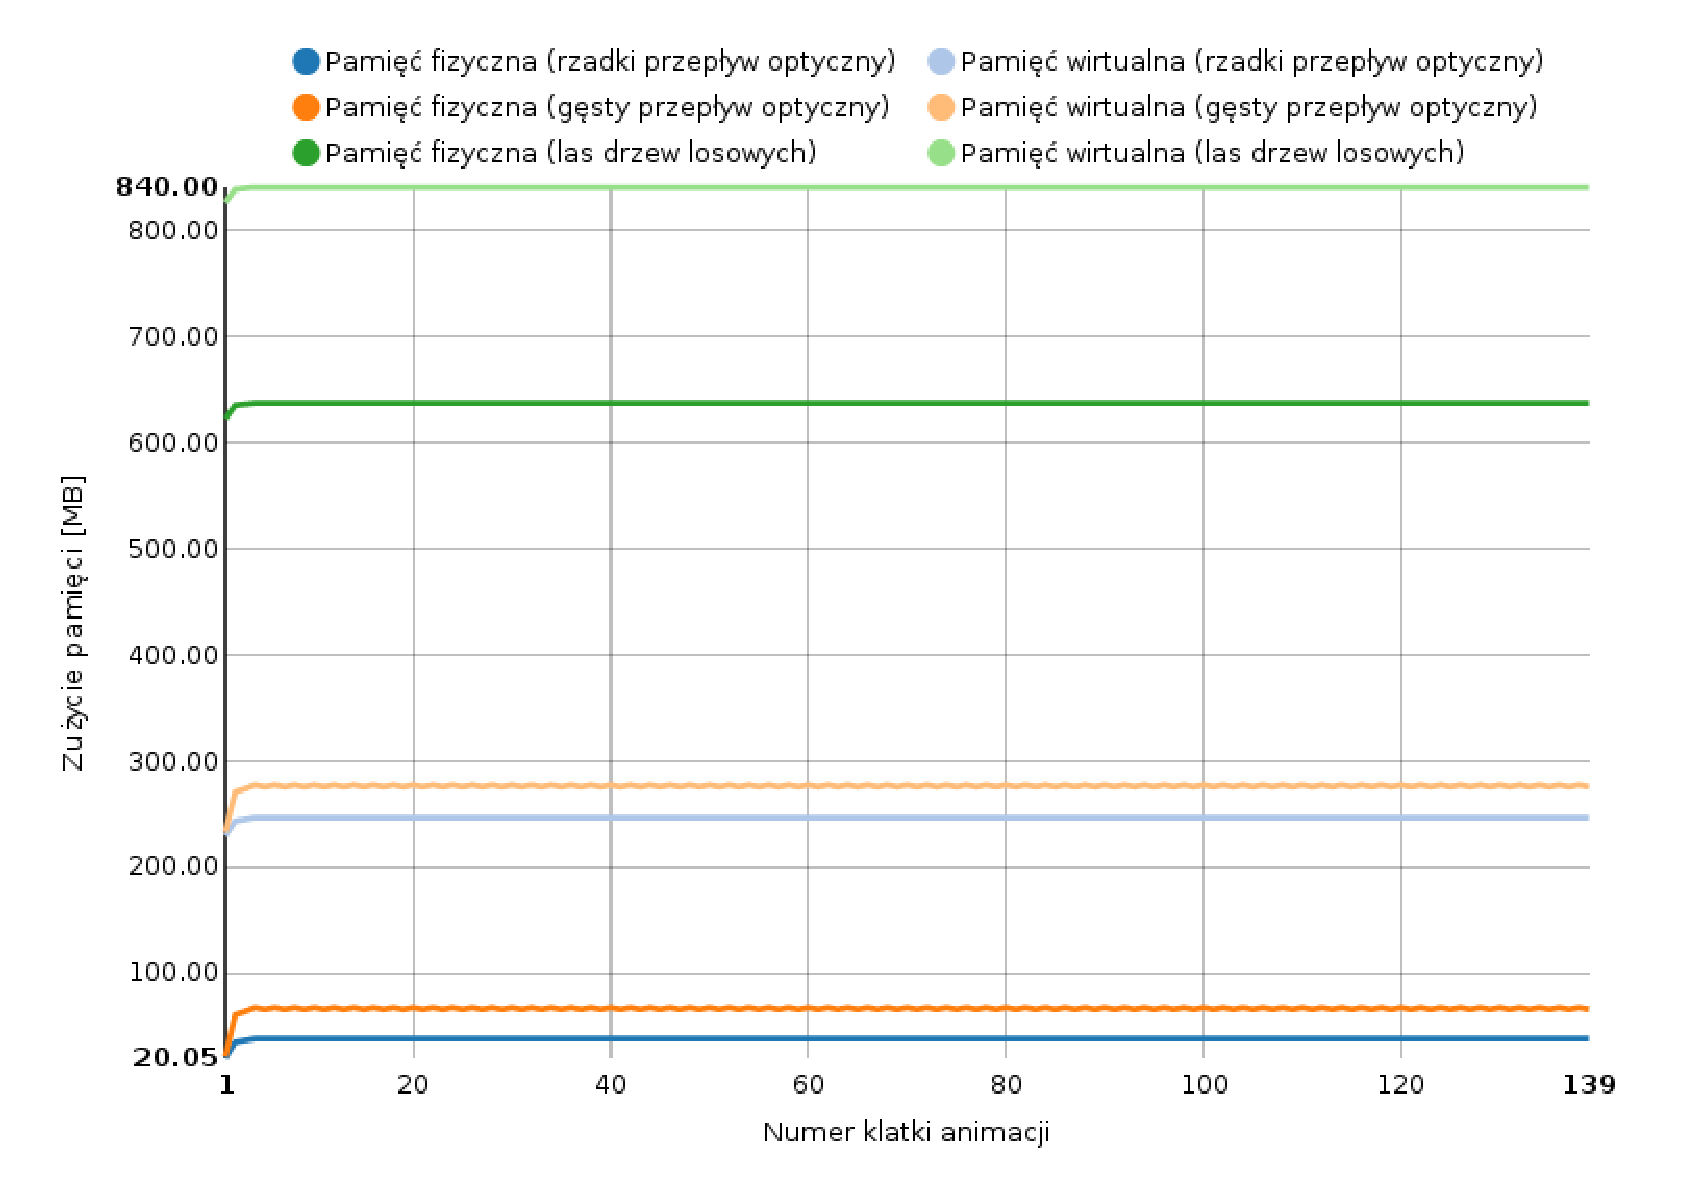
\includegraphics[width=14cm]{charts/memory/PersonAC}
      \caption[Wykres zużycia pamięci dla próbki o nazwie Person\_A\_C]
              {Wykres zużycia pamięci dla próbki o nazwie \textit{Person\_A\_C}}
      \label{fig:MemoryUsagePersonAC}
    \end{figure}

    W~przypadku gęstego przepływu optycznego zużycie pamięci fizycznej nie przekracza $80$ MB, dla implementacji algorytmu opartego o~metodę \textit{LK} osiąga wartość co najwyżej $50$ MB. Oba algorytmy są zdecydowanie oszczędniejsze od trzeciej zapronowanej implementacji.

    \begin{figure}[!ht]
      \centering
      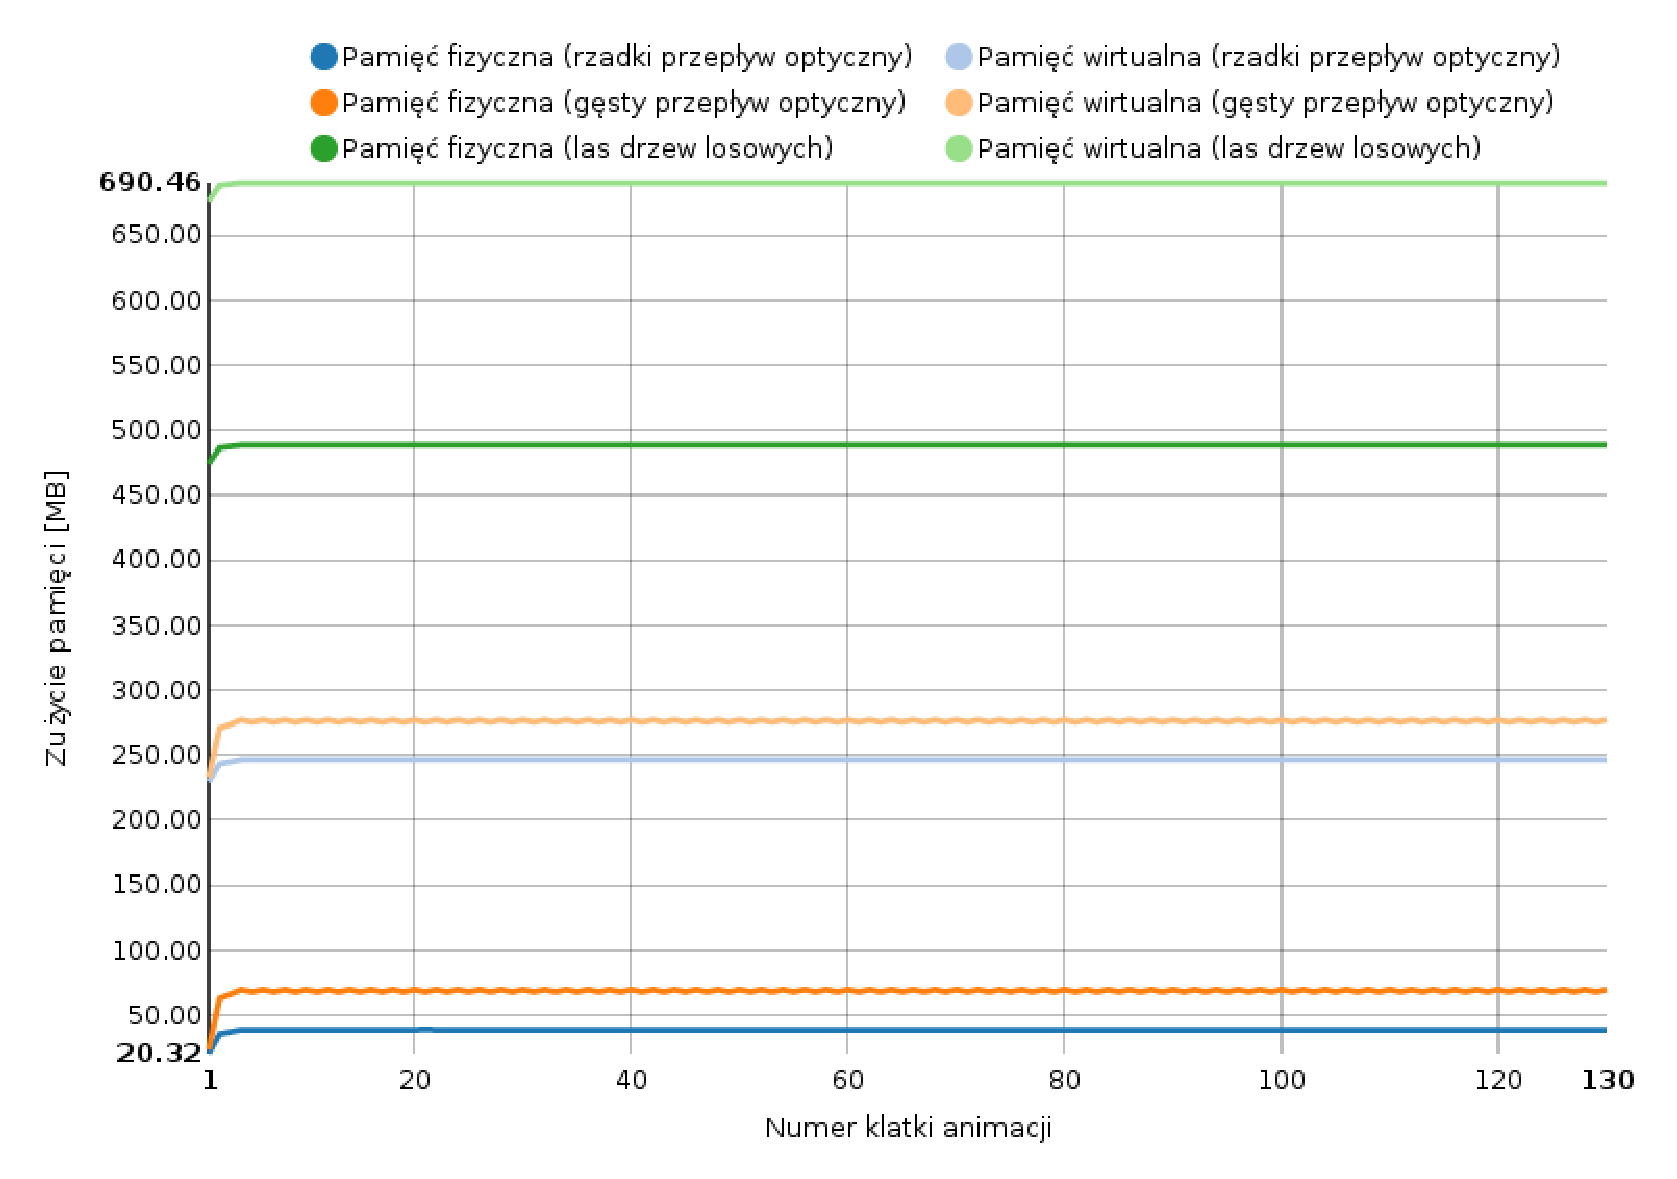
\includegraphics[width=14cm]{charts/memory/PersonGC}
      \caption[Wykres zużycia pamięci dla próbki o nazwie Person\_G\_C]
              {Wykres zużycia pamięci dla próbki o nazwie \textit{Person\_G\_C}}
      \label{fig:MemoryUsagePersonGC}
    \end{figure}

    Algorytm gęstego przepływu optycznego posiada jedną wadę - mimo stosunkowo niewielkiego zużycia pamięci, na wykresie \ref{fig:OpticalFlowsMemoryUsage} został zaprezentowany piłokształtny przebieg, ciągłej alokacji i~zwalniania od 2 do 4 MB bufora pamięci pomiędzy poszczególnymi klatkami sekwencji wideo. Nie jest to korzystne zjawisko i~jego eliminacja na pewno wpłynie pozytywnie na całkowitą wydajność.

    \begin{figure}[!ht]
      \centering
      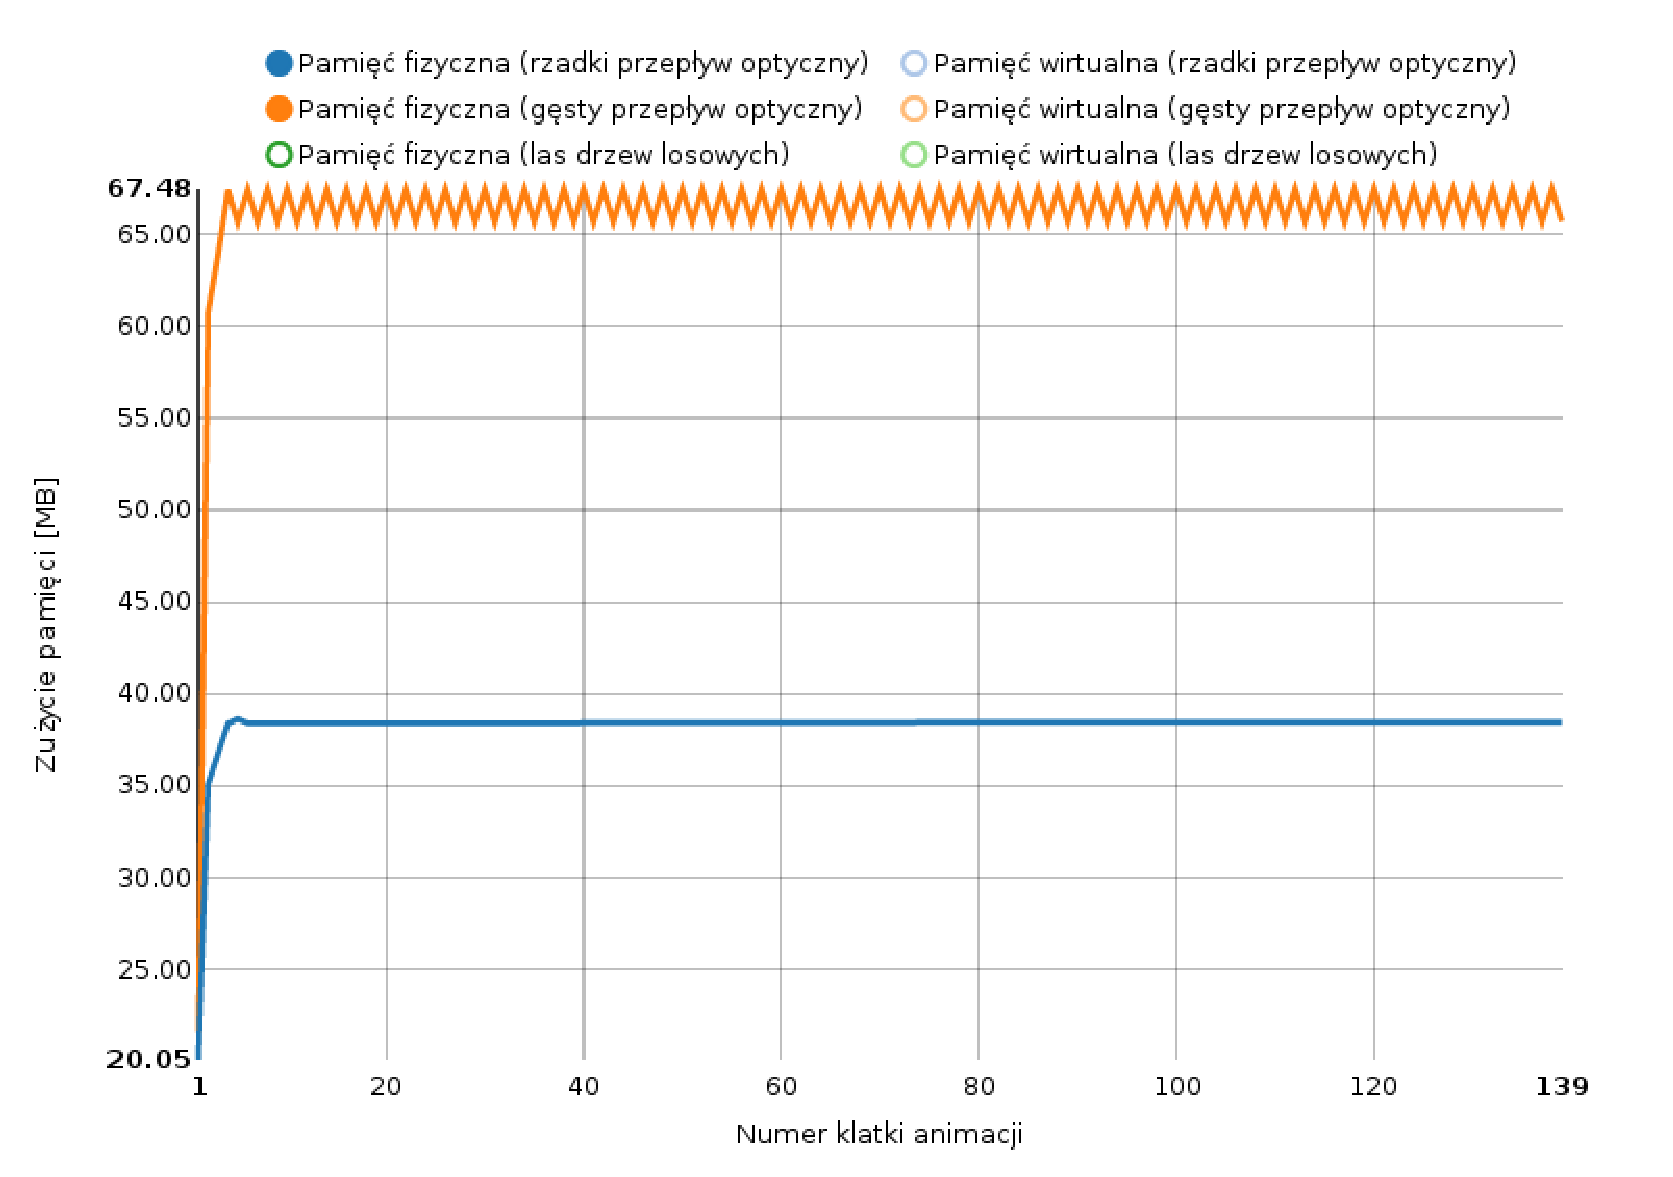
\includegraphics[width=14cm]{charts/memory/OpticalFlows}
      \caption[Wykres zużycia pamięci dla algorytmów przepływu optycznego]
              {Wykres zużycia pamięci dla algorytmów przepływu optycznego}
      \label{fig:OpticalFlowsMemoryUsage}
    \end{figure}

    W~przypadku algorytmu opartego o~las drzew losowych zużycie pamięci liniowo zależy od ilości wytrenowanych drzew wykorzystanych do budowy klasyfikatora. Zależność została zaprezentowana na rysunku \ref{fig:RandomForestTrackerPerTrainedTreesAmount}. Jednocześnie można zauważyć, że różnica pomiędzy minimalnym i~maksymalnym zużyciem pamięci jest niewielka co oznacza, że proces potrzebuje dużej ilości pamięci, ale nie jest algorytmem intensywnym w~operacje przydzielania i~zwalniania zasobów.

    \begin{figure}[!ht]
      \centering
      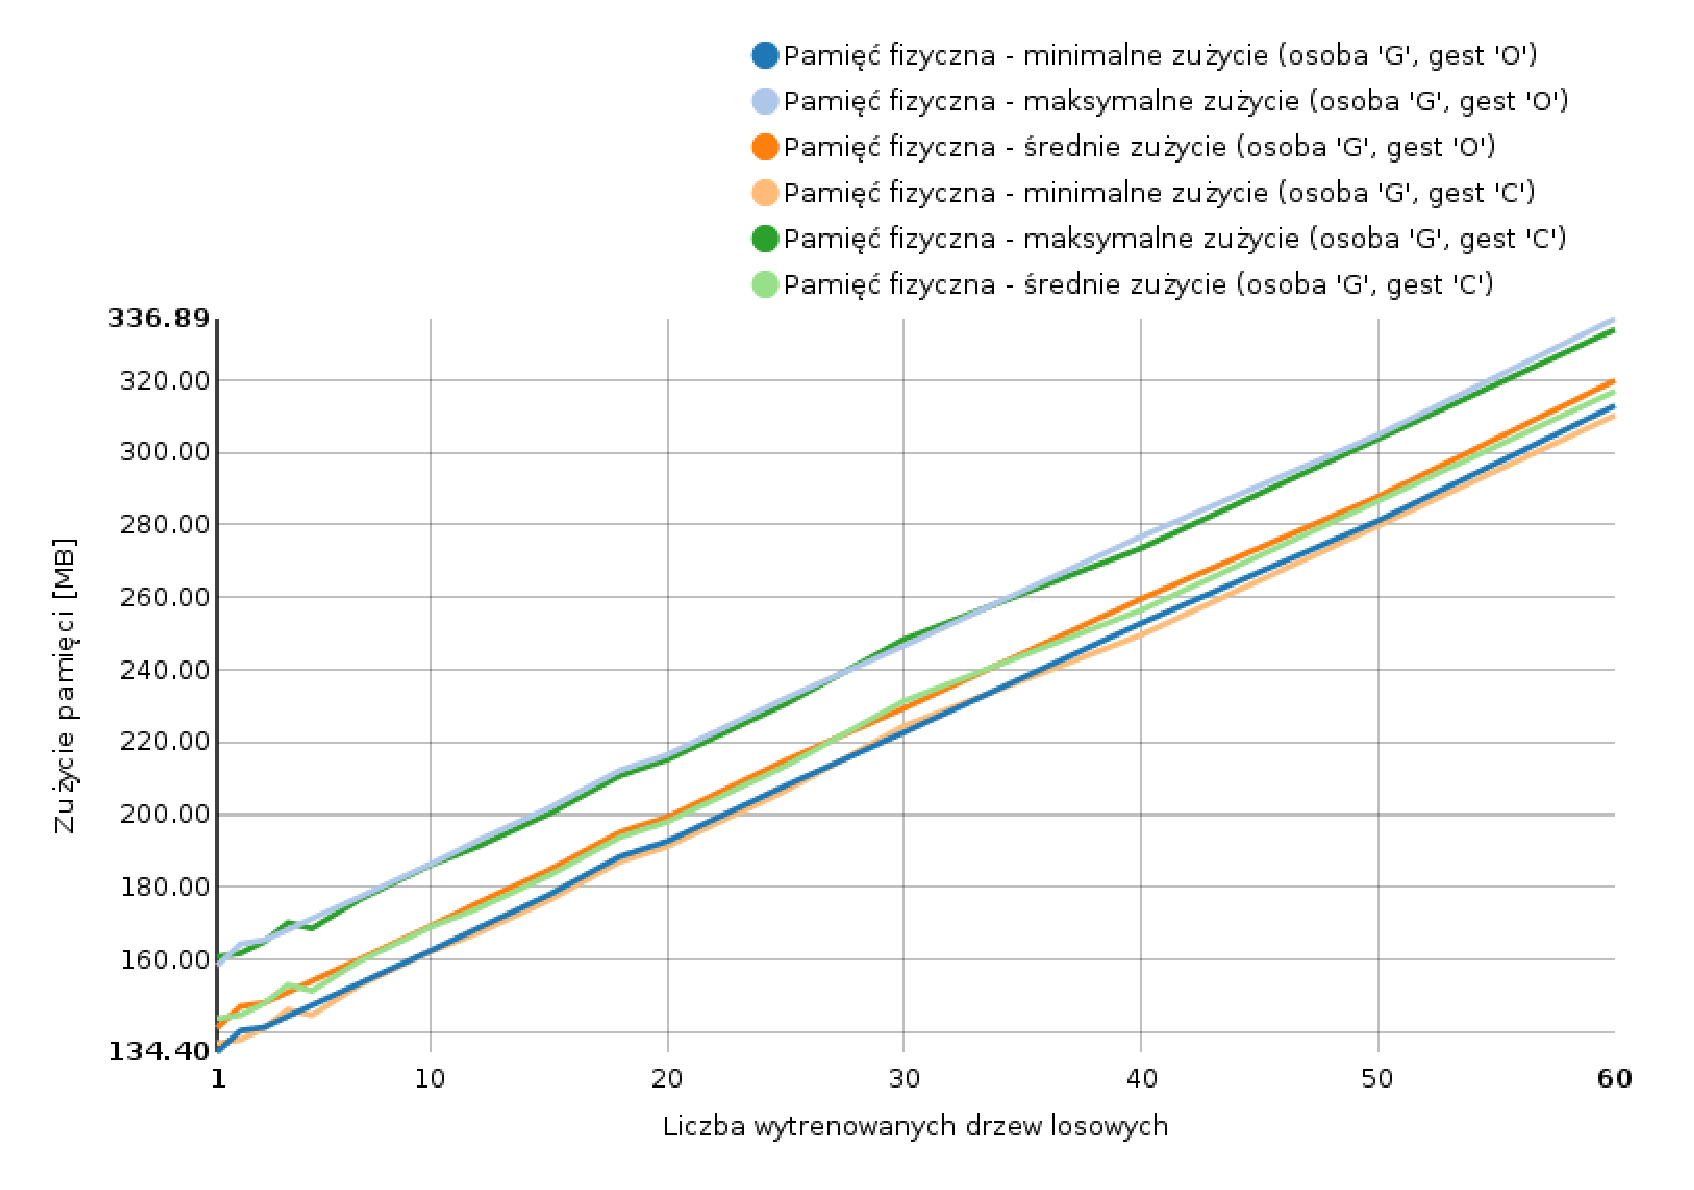
\includegraphics[width=14cm]{charts/memory/RandomPerTrainedTree}
      \caption[Wykres zużycia pamięci dla algorytmu lasu drzew losowych w~zależności od liczby wytrenowanych drzew]
              {Wykres zużycia pamięci dla algorytmu lasu drzew losowych w~zależności od liczby wytrenowanych drzew}
      \label{fig:RandomForestTrackerPerTrainedTreesAmount}
    \end{figure}

    Rzadki przepływ optyczny charakteryzuje się niewielkimi wahaniami zużycia pamięci w~zależności od minimalnej odległości pomiędzy śledzonymi punktami charakterystycznymi (jak można było przypuszczać, im większa odległość tym mniejsze zużycie pamięci). Na wykresie \ref{fig:SparseOpticalFlowPerMinimalDistanceBetweenPoints} widać, że fluktuacje mieszczą się w~przedziale o~szerokości około $30$ MB i~nie przekraczają wartości $63$ MB, co nie jest bez znaczenia w~środowisku z~ograniczonymi zasobami pamięciowymi (np. systemy wbudowane lub urządzenia mobilne). Z trzech porównywanych implementacji, metoda oparta o~algorytm \textit{LK} w~wariancie piramidalnym jest najoptymalniejsza pod względem zużycia pamięci.

    \begin{figure}[!ht]
      \centering
      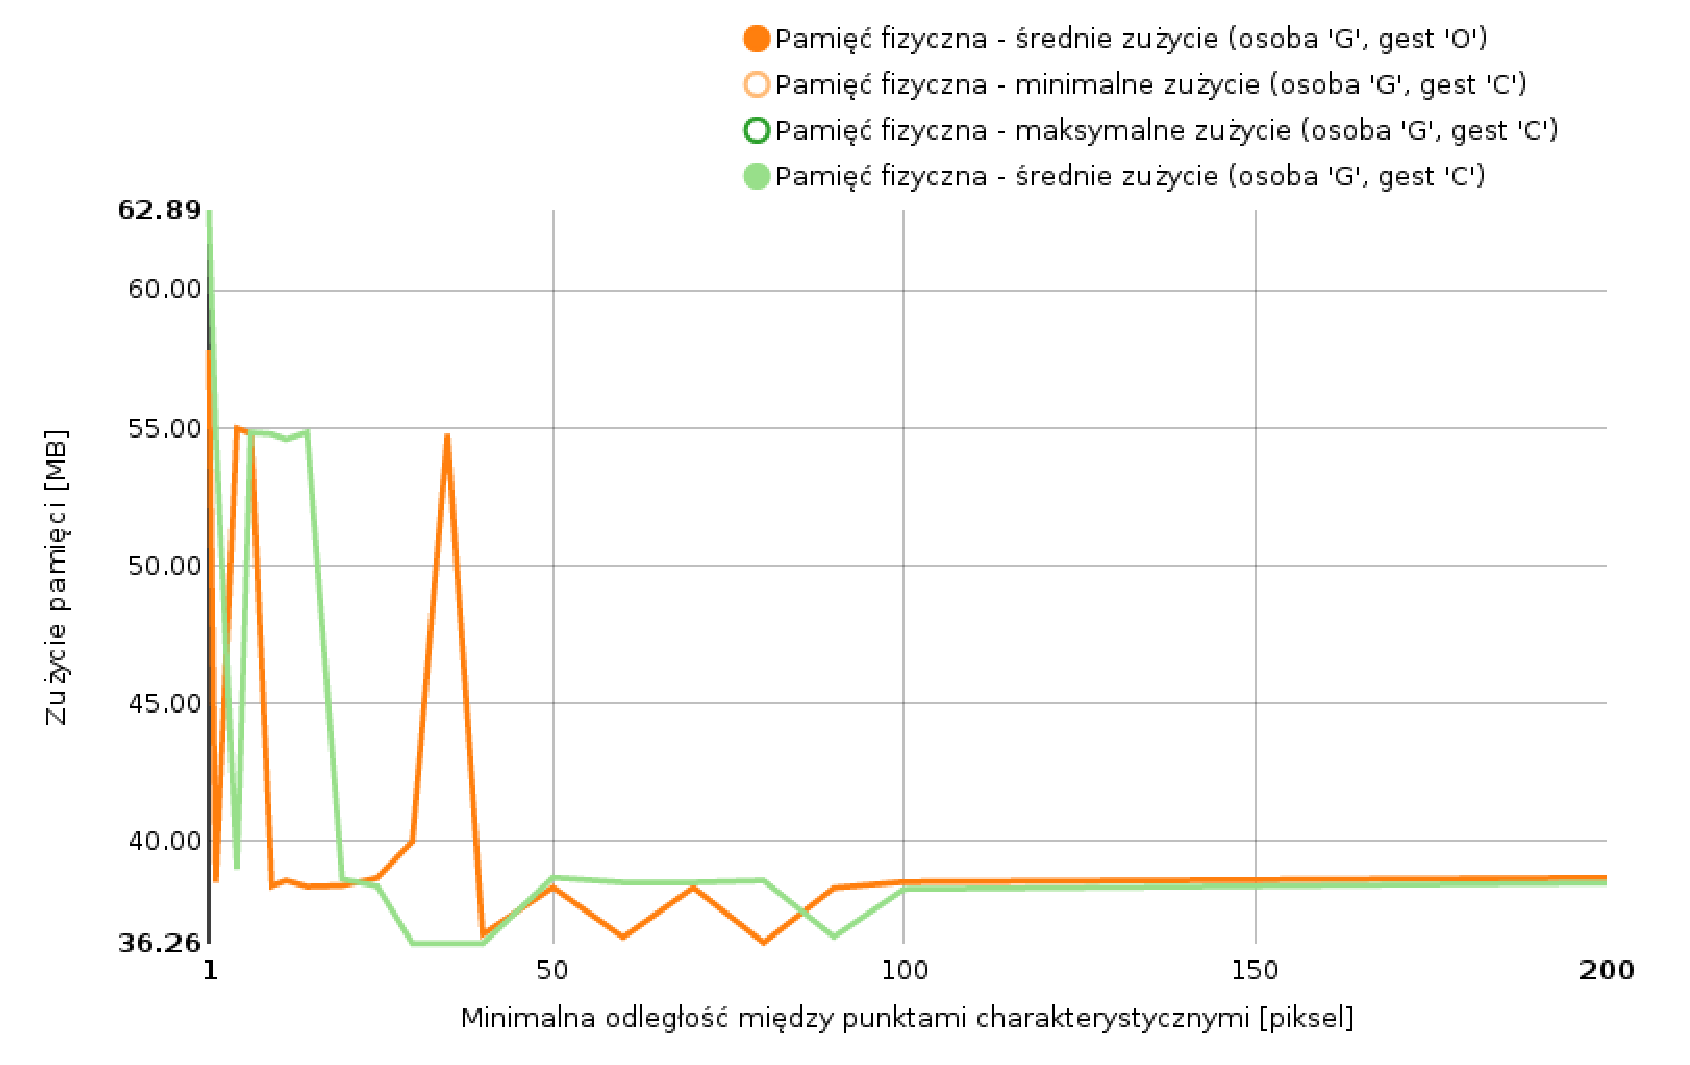
\includegraphics[width=14cm]{charts/memory/SparsePerMinimalDistance}
      \caption[Wykres zużycia pamięci dla rzadkiego przepływu optycznego w~zależności przyjętej minimalnej odległości pomiędzy punktami charakterystycznymi]
              {Wykres zużycia pamięci dla rzadkiego przepływu optycznego w~zależności przyjętej minimalnej odległości pomiędzy punktami charakterystycznymi}
      \label{fig:SparseOpticalFlowPerMinimalDistanceBetweenPoints}
    \end{figure}

    \begin{figure}[!ht]
      \centering
      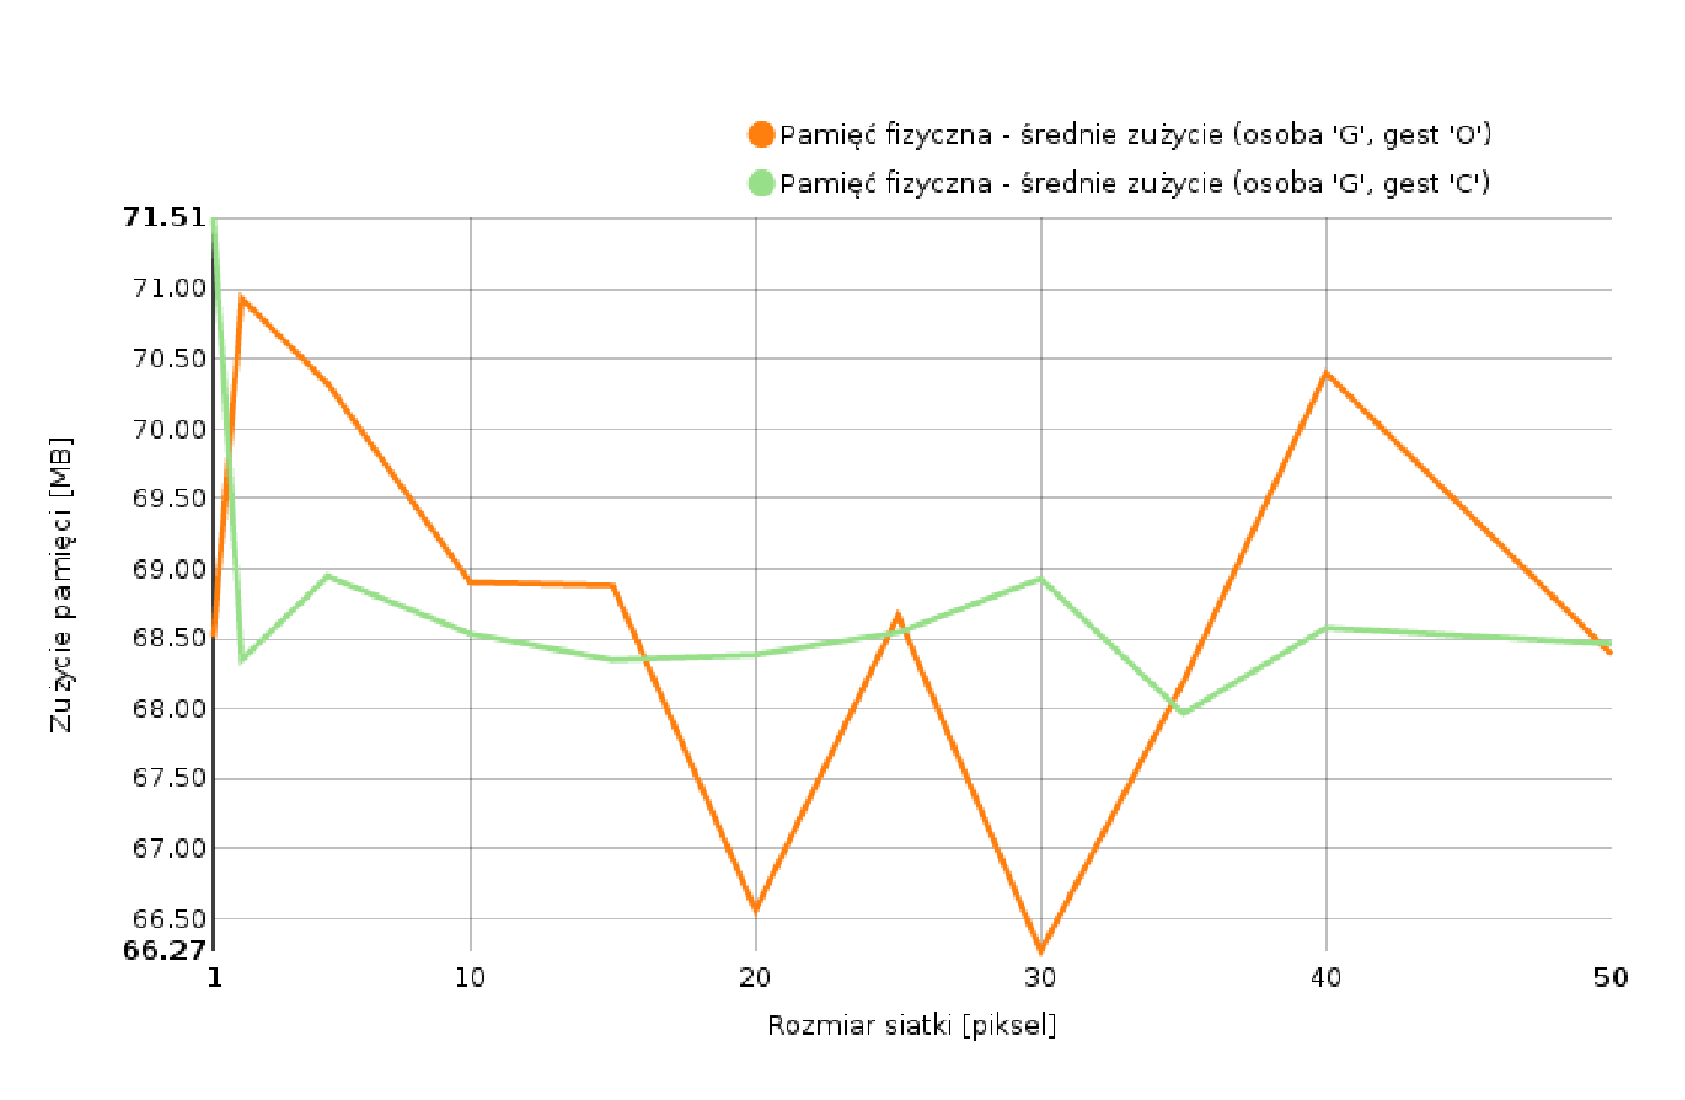
\includegraphics[width=14cm]{charts/memory/DensePerMapOverlaySize}
      \caption[Wykres zużycia pamięci dla gęstego przepływu optycznego w~zależności od gęstości siatki]
              {Wykres zużycia pamięci dla gęstego przepływu optycznego w~zależności od gęstości siatki}
      \label{fig:DenseOpticalFlowPerMapSize}
    \end{figure}

    \newpage

    W~wariancie gęstym zależnym od rozmiaru przyjętej siatki, przepływ optyczny charakteryzuje się wyższym zużyciem pamięci (maksymalnie około $72$ MB), jednak same wahania są stabilniejsze, mieszczą się w~przedziale o~szerokości około $5$ MB. Widać, że zwiększenie wymiarów siatki (intuicyjnie, rozrzedzenie jej) nie zawsze idzie w~parze z~malejącym zużyciem pamięci. Warto jednak zauważyć, że wahania odbywają sie w~bardzo niewielkim zakresie.

    Mimo wyższego zużycia całościowego, jego wartość nadal nie jest zbyt wysoka i~algorytm gęstego przepływu optycznego sprawdzi się w~środowisku z~ograniczonymi zasobami pamięciowymi.

  \section{Wnioski i~wyniki badania wydajności}\label{Section_Timing}

  \section{Wnioski i~wyniki związane z~wprowadzonym narzutem czasowym}\label{Section_Overhead}

  \section{Wyniki i~wnioski weryfikacji jakości badanych algorytmów}\label{Section_Quality}

  \section{Proponowane usprawnienia}\label{Section_Usprawnienia}

    Na podstawie analizy zawartej w~powyższych podrozdziałach nasuwa się kilka wniosków i~potencjalnych ulepszeń. Zostały one zebrane i~omówione poniżej.

    \begin{itemize}
      \item \textbf{Rozszerzenie sposobu budowania bazy treningowej dla algorytmu wykorzystującego las drzew losowych.}

      Aby zwiększyć jakość klasyfikacji oraz jeszcze bardziej uodpornić algorytm na zmianę kształtu śledzonej dłoni należy udoskonalić proces generacji danych wejściowych. Potencjalnym rozszerzeniem może być wykorzystanie nie tylko pierwszej klatki animacji, do generowania zbioru danych treningowych. Innym rozszerzeniem, może być dodanie kolejnych transformacji źródłowej klatki animacji (np. celowego zniekształcenia perspektywy lub tzw. \textit{rybiego oka} oraz dodatkowego rodzaju szumu).

      \item \textbf{Optymalizacja zużycia pamięci dla algorytmu przepływu optycznego gęstego.}

      W~sekcji \ref{Section_Memory} podczas omawiania zużycia pamięci dla wspomnianego algorytmu dało się zauważyć ciągłą zmianę zużywanej pamięci fizycznej (i~w konsekwencji także wirtualnej, rysunek \ref{fig:OpticalFlowsMemoryUsage}). Ciągła alokacja i~zwalnianie przydzielonych zasobów negatywnie wpływa na czas przetwarzania klatki sekwencji wideo. Narzut ten, może zostać zniwelowany za pomocą zmiany sposobu alokacji pamięci np. poprzez zastosowanie wielokrotnie wykorzystywanej i~współdzielonej puli pamięci.

      \item \textbf{Optymalizacja zużycia pamięci dla algorytmu opartego o drzewa losowe.}

      Omawiany algorytm podczas pracy wykorzystuje bardzo dużo (w~odniesieniu do pozostałych dwóch metod) pamięci fizycznej. W~celu zwiększenia przydatności algorytmu należy przeprowadzić proces optymalizacji zużycia pamięci.

      \item \textbf{Przyspieszenie procesu uczenia, odczytu oraz zapisu bazy treningowej.}

       W~obecnej implementacji przy generacji, zapisie oraz odczycie bazy treningowej wykorzystywany jest jeden wątek (w~konsekwencji również jeden procesor). W~oryginalnym algorytmie (opisanym w~pracy \cite{RandomizedTrees06}) autorzy proponują rozdzielenie omawianych etapów pracy algorytmu na cztery wątki, co zdecydowanie lepiej wykorzystuje możliwości współczesnego sprzętu.
    \end{itemize}

\chapter{Podsumowanie}\label{Section_Podsumowanie}

W~ramach pracy magisterskiej omówiono i~przeprowadzono badania wydajnościowe oraz jakościowe implementacji trzech algorytmów śledzenia punktów charakterystycznych pod kątem wykorzystania ich do analizy ruchu dłoni.

Zebrane rezultaty pozwoliły na jednoznaczne określenie przydatności poszczególnych algorytmów w~badanym obszarze.

Oprócz zaproponowanych implementacji, badań oraz~analizy zostały również zaproponowane usprawnienia i~potencjalne rozszerzenia, które zwiększą jakość oraz poprawia wydajność omawianych metod.